\documentclass[12pt,a4paper]{article}
\usepackage{graphics}
\usepackage{amssymb}
\usepackage{ragged2e}
\justifying
\usepackage[utf8]{inputenc}
\usepackage[russian]{babel}
\usepackage[width=17cm,top=1cm,height=27cm]{geometry}
\usepackage{graphicx}
\title{Численные методы(Мусаева)}

\date{November 2019}

\begin{document}
\begin{titlepage}
\begin{center}
2019 год
\vspace {8cm}



{ \LARGEПрактикум по численным методам:\\ интерполирование функций }\\
\vspace {8cm}
\bigskip Мусаева Аида, группа 301
\end{center}
\vfill
\vfill
\end{titlepage}

\section{Полином Лагранжа}
\text{
На отрезке $[-10, 10] \subset \mathbb{R}$ рассматривается функция $f(x) = x^2cos 2x + 1$ и известны её значения в $(n+1)$ различных узлах $x_0, x_1,\ldots, x_n$, принадлежащих $[-10, 10]$. Искомый интерполяционный \textit{полином Лагранжа}: \\
\begin{displaymath}
    L_n(x) = \sum_{i=0}^n f(x_i)l_i(x),
\end{displaymath}
  где $l_k(x) = \frac{(x - x_o)\cdots(x-x_{k-1})(x-x_{k+1})\cdots(x_k-x_n)}{(x_k - x_o)\cdots(x_k-x_{k-1})(x_k-x_{k+1})\cdots(x_k-x_n)}$ \\\\
\subsection{Полином Лагранжа с равноотстоящими узлами интерполирования}
Пусть $(n + 1) = 11$ - количество равноотстоящих узлов. \\\\
Найдём интерполяционный полином Лагранжа и построим графики:
}
\subsubsection{Код программы:}
\begin{verbatim}
import numpy as np
import matplotlib.pyplot as plt
from sympy import *


def f(x):
    return (x ** 2) * np.cos(2 * x) + 1

def pLagrange(X, Y):
    x = symbols('x')
    L = 0
    for j in range(np.prod(X.shape)):
        l = 1
        l_j = 1
        for i in range(np.prod(X.shape)):
            if i == j:
                l *= 1
                l_j *= 1
            else:
                l *= (x - X[i])
                l_j *= (X[j] - X[i])
        L += Y[j] * l / l_j
    return collect(expand(L), x)

def makeData(func,n = 10, a = -10, b = 10):
    X = np.arange(a, b + 1, (b - a) / n)
    Y = np.array(func(X))
    return X, Y

x = symbols('x')
L = pLagrange(makeData(f)[0], makeData(f)[1])
print(L)

xnew = np.arange(-10, 11, 0.01)
dot = makeData(f)
fig, ax = plt.subplots()
ax.set_ylim([-250, 150])
line1, = ax.plot(xnew, f(xnew),
                 label='f(x)')

line2, = ax.plot(xnew, [L.subs(x, xnew[i]) for i in range(np.prod(xnew.shape))],
                 label='Lagrange polynomial')
line3 = plt.plot(dot[0], dot[1], marker='o', color='k', ls='')
ax.legend(loc='upper left')
plt.show()
\end{verbatim}

\subsubsection{Результат работы программы}
\begin{verbatim}
L(x) = 9.42467373706769e-7*x**10 - 0.000156322149555344*x**8 + 
+ 0.00675993213419734*x**6 - 0.0454561240250664*x**4 - 
- 0.570214692986631*x**2 + 1.0
\end{verbatim}

\begin{figure}[h]
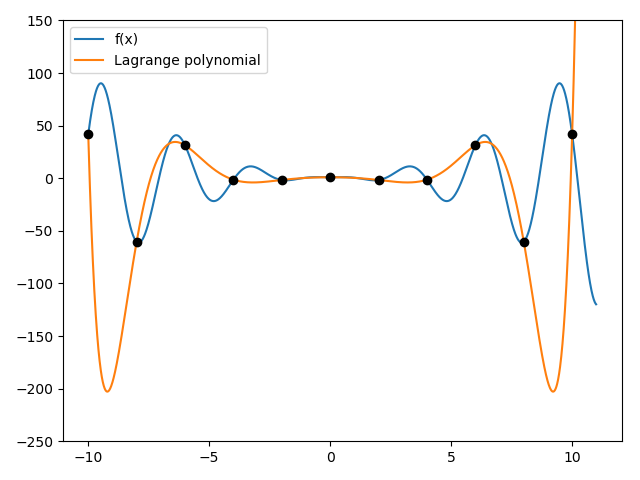
\includegraphics[width=\linewidth]{L(f)1.PNG}
\caption{}
\label{fig:}
\end{figure}
\vspace{5cm}
\subsection{Выбор узлов интерполяции}
\text{Рассмотрим множество $F_n$ всевозможных функций $f$, которые $(n+ 1)$ раз непрерывно дифференцируемы на $[a, b]$ и производная которых порядка $(n+ 1)$ ограничена по модулю числом $M_{n+1}: |f^{(n+1)}(x)| \leq M_{n+1}, x \in [a,b]$. В этом классе функций остаток интерполирования (методическая погрешность интерполирования) имеет оценку:\\
$|r_n(x)| \leq \frac{M_{n+1}}{(n+1)!}\omega_{n+1}(x)$,\\
где $\omega_{n+1}(x) = |x - x_0||x - x_1| \ldots |x-x_n|$\\\\
Множитель $\frac{M_{n+1}}{(n+1)!}$ не зависит от выбора узлов, поэтому при фиксированном значении $\overline{x}$ необходимо выбрать {$\overline{x_{i_k}}$} так, чтобы $|\overline{x} - x_0||\overline{x} - x_1| \ldots |\overline{x}-x_n|$ имело наименьшее значение. \\
Эта величина принимает наименьшее возможное значение, если узлы интерполяции являются корнями полинома Чебышева степени $n+1$:\\
$x_i = \frac{1}{2}[(b - a)*cos(\pi \frac{2i+1}{2(n+1)}) + (b+a)]$, $i = \overline{0, n}$
}

\subsubsection{Код программы:}
\begin{verbatim}
def f(x):...
def pLagrange(X, Y):...
def makeData(func, flag = 'equidistant', n = 10, a = -10, b = 10):
    if flag == 'equidistant':
        X = np.arange(a, b + 1, (b - a) / n)
        Y = np.array(func(X))
        return X, Y
    elif flag == 'minError':
        X = np.array([((b/2-a/2)*math.cos((2*i+1)*math.pi/(2*n+2)) + (b+a)/2) 
            for i in range(n+1)])
        Y = np.array(func(X))
        return X, Y
    print('Incorrect flag')
    return -1

x = symbols('x')
dot = makeData(f, 'minError')
L = pLagrange(dot[0], dot[1])
print(L)

xnew = np.arange(-10, 11, 0.01)
fig, ax = plt.subplots()

ax.set_ylim([-250, 150])
line1, = ax.plot(xnew, f(xnew),
                 label='f(x)')

line2, = ax.plot(xnew, [L.subs(x, xnew[i]) for i in range(np.prod(xnew.shape))],
                 label='Lagrange polynomial')

line3 = plt.plot(dot[0], dot[1], marker='o', color='k', ls='')
ax.legend(loc='upper left')
plt.show()
\end{verbatim}

\subsubsection{Результат работы программы}:
\begin{verbatim}
L(x) = -7.36389334252906e-7*x**10 - 1.89920962440019e-20*x**9 +
+ 0.000145779716813414*x**8 + 4.91618674708876e-18*x**7 - 0.00847010385653533*x**6 -
- 3.2580443758625e-16*x**5 + 0.126393162403064*x**4 + 1.15463194561016e-14*x**3 + 
+ 0.257396729645615*x**2 - 6.26445190060953e-14*x + 1.0
\end{verbatim}

\begin{figure}
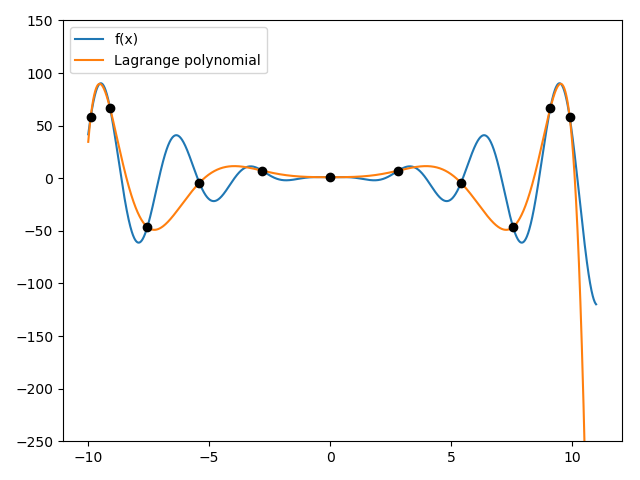
\includegraphics[width=\linewidth]{L(f)2.png}
\caption{}
\label{fig:}
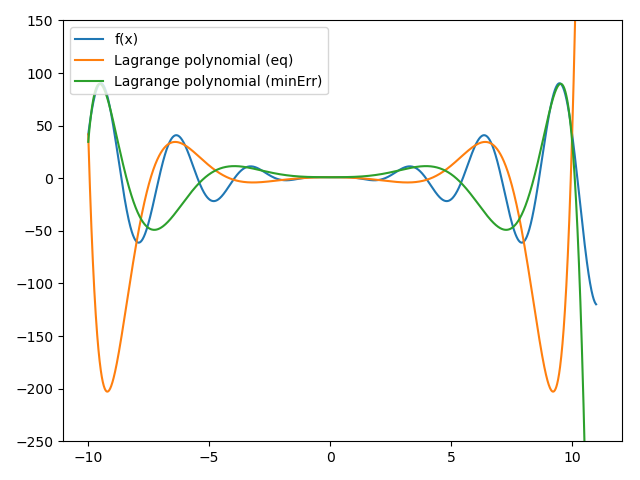
\includegraphics[width=\linewidth]{compar1.png}
\caption{}
\label{fig:}
\end{figure}\\

\vspace{190cm}
\subsection{Увеличение количества узлов}
\text{Увеличим количество интерполяционных узлов до $(n+1) = 15$
}

\subsubsection{Код программы:}
\begin{verbatim}
def f(x):...
def pLagrange(X, Y):...
def makeData(func, flag = 'equidistant', n = 10, a = -10, b = 10):...
x = symbols('x')
dot = makeData(f, 'equidistant', 14)
L1 = pLagrange(dot[0], dot[1])
print(L1)

dot = makeData(f, 'minError', 14)
L2 = pLagrange(dot[0], dot[1])
print(L2)

xnew = np.arange(-10, 11, 0.01)

fig, ax = plt.subplots()
ax.set_ylim([-250, 150])
line1, = ax.plot(xnew, f(xnew),
                 label='f(x)')

line2, = ax.plot(xnew, [L1.subs(x, xnew[i]) for i in range(np.prod(xnew.shape))],
                 label='Lagrange polynomial (eq)')
line3 = ax.plot(xnew, [L2.subs(x, xnew[i]) for i in range(np.prod(xnew.shape))],
                 label='Lagrange polynomial (minErr)')
ax.legend(loc='upper left')
plt.show()

\end{verbatim}
\textbf{Результат работы программы}:\\
\begin{verbatim}
L(eq) = -5.79327235589803e-9*x**14 + 9.46087825607525e-24*x**13 +
1.57275377813924e-6*x**12 - 3.30607547225194e-20*x**11 - 0.000158191730507908*x**10 - 
7.30142400533207e-19*x**9 + 0.00732118600907543*x**8 + 5.77879757934774e-17*x**7 
- 0.1568734516899*x**6 - 4.35415592470179e-16*x**5 + 1.36005833713142*x**4 
+ 5.07927033766009e-15*x**3 - 3.14161853128291*x**2 - 2.06501482580279e-14*x + 1.0 

L(minErr) = 5.46067751932958e-10*x**14 + 1.31444169213505e-23*x**13
- 1.9991104546399e-7*x**12 - 3.99693671985623e-21*x**11 +
2.74394926899682e-5*x**10 + 6.38662842229742e-19*x**9 - 0.00174033620621009*x**8
- 5.96311194867027e-18*x**7 + 0.0503234631744972*x**6 + 1.36349265211777e-15*x**5 
- 0.544458975436801*x**4 - 1.38500322321988e-14*x**3 + 1.01827155368013*x**2
+ 4.00790511889682e-14*x + 1.0
\end{verbatim}
\begin{figure}[h]
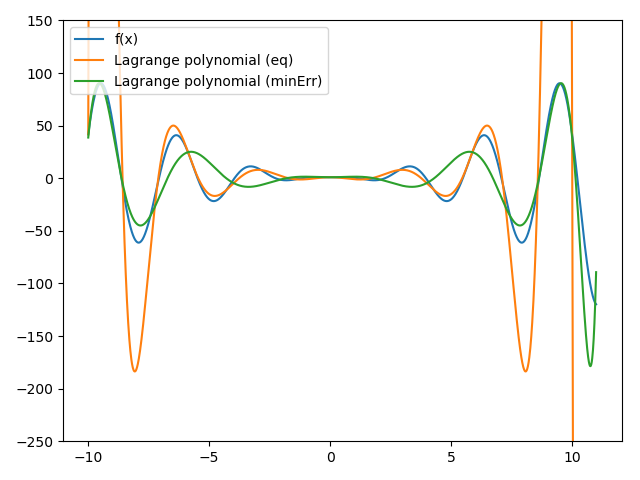
\includegraphics[width=\linewidth]{compar2.png}
\caption{}
\label{fig:}
\end{figure}\\

\vspace{20cm}
\subsection{Постановка задачи}
\text{Построить интерполяционные полиномы Лагранжа для функции $h(x) = |x|f(x)$ и сравнить их поведение на промежутке $[-10,10]$. Пусть $(n+1) = 15$}
\subsubsection{Код программы:}
\begin{verbatim}
def f(x):...
def pLagrange(X, Y):...
def makeData(func, flag = 'equidistant', n = 10, a = -10, b = 10):...
def plotCompare(func, L1, L2):
    xnew = np.arange(-10, 11, 0.01)
    fig1, ax = plt.subplots()
    if func.__name__ == "h":
        ax.set_ylim([-2500, 2500])
    else:
        ax.set_ylim([-250, 250])
    line1, = ax.plot(xnew, func(xnew),
                     label=func.__name__+ "(x)")

    line2, = ax.plot(xnew, [L1.subs(x, xnew[i]) for i in range(np.prod(xnew.shape))],
                     label='Lagrange polynomial (eq)')
    line3 = ax.plot(xnew, [L2.subs(x, xnew[i]) for i in range(np.prod(xnew.shape))],
                    label='Lagrange polynomial (minErr)')
    ax.legend(loc='upper left')
    plt.show()

x = symbols('x')
dot1 = makeData(h, 'equidistant', 14)
L1 = pLagrange(dot1[0], dot1[1])
print(L1)
dot2 = makeData(h, 'minError', 14)
L2 = pLagrange(dot2[0], dot2[1])
print(L2)
plotCompare(h, L1, L2)
\end{verbatim}
\textbf{Результат работы программы}:\\
\begin{verbatim}
L(eq) = -2.02322265230865e-8*x**14 - 1.78671012311454e-22*x**13 + 5.41593316431182e-6*x**12 - 5.84452733605467e-20*x**11 - 0.000532799424310911*x**10 - 8.34835672813838e-18*x**9 + 0.0237920042172422*x**8 + 3.85108611666851e-16*x**7 - 0.480177094782046*x**6 - 5.49560397189452e-15*x**5 + 3.73266994095506*x**4 + 3.86357612569554e-14*x**3 - 6.48213183954967*x**2 - 9.68114477473137e-14*x + 1.77635683940045e-15 
L(minErr) = 2.44660815833163e-9*x**14 + 8.58846120377323e-23*x**13 - 9.89511616076375e-7*x**12 - 2.89810999414079e-20*x**11 + 0.000145789409145056*x**10 + 3.93319749057534e-18*x**9 - 0.0097343234743911*x**8 - 6.41847686111419e-17*x**7 + 0.293869006573631*x**6 + 7.7559486610923e-15*x**5 - 3.40498864536367*x**4 - 7.57449658550513e-14*x**3 + 9.35135591096702*x**2 + 2.37143638059933e-13*x + 2.83276944882323e-15
\end{verbatim}
\begin{figure}[h]
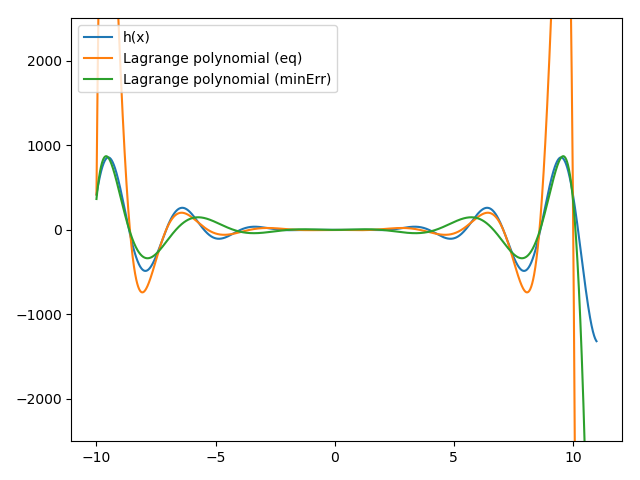
\includegraphics[width=\linewidth]{L(h).png}
\caption{}
\label{fig:}
\end{figure}\\

\end{document}
